% When something goes wrong – Training 3 slides
% Build: latexmk -lualatex 60-minute-training.tex   (or: lualatex 60-minute-training.tex)
% Authors: Divya Ravichandran, Álvaro Gómez García, Mohammed Krayem (University of Luxembourg)
% Speaker notes: change "hide notes" to "show notes on second screen=right" below.
\documentclass[aspectratio=169,11pt,t]{beamer}
\usetheme{focus}
\usepackage{qrcode}
\usetikzlibrary{arrows.meta}
\setbeameroption{hide notes}

% ---- Slide helpers ----
% \statement{<colour>}{<icon>}{<text>}: one card of the warm-up list
\newcommand\statement[3]{%
  \begin{card}[left=3mm, top=1.1mm, bottom=1.1mm]
    \iconbadge[8mm]{#1}{#2}\hspace{3mm}\begin{minipage}[c]{.84\linewidth}\raggedright\mediumfont\small #3\end{minipage}
  \end{card}\vspace{-1.5mm}}
% \trainer{<colour>}{<initials>}{<name>}: one card of "Who we are" (no photo, initials avatar)
\newcommand\trainer[3]{%
  \begin{card}[equal height group=trainers, before upper=\centering, top=3mm, bottom=3mm]
    \tikz\node[circle, fill=#1, text=white, minimum size=12mm, font=\headfont\large]{#2};\par\vspace{2mm}
    {\headfont\color{navy}#3}
  \end{card}}
% \takeaway{<colour>}{<icon>}{<title>}{<text>}: one card of "what you will take home"
\newcommand\takeaway[4]{%
  \begin{card}[equal height group=takeaway, before upper=\centering, top=3mm, bottom=3mm]
    \iconbadge[10mm]{#1}{#2}\par\vspace{2mm}
    {\headfont\large\color{navy}#3}\par\vspace{1.5mm}
    {\small\color{muted}#4}
  \end{card}}

% \step{<colour>}{<n>}{<text>}: numbered step card
\newcommand\step[3]{%
  \begin{card}[left=3mm, top=1.3mm, bottom=1.3mm, before skip=0pt, after skip=2.2mm]
    \iconbadge[7.5mm]{#1}{\headfont #2}\hspace{3mm}\begin{minipage}[c]{.84\linewidth}\raggedright\mediumfont\small #3\end{minipage}
  \end{card}}

% \gstep{<colour>}{<n>}{<text>}: compact numbered step for narrow columns
\newcommand\gstep[3]{%
  \begin{card}[left=2.5mm, top=1.2mm, bottom=1.2mm, before skip=0pt, after skip=1.8mm]
    \iconbadge[6.5mm]{#1}{\headfont\small #2}\hspace{2.5mm}\begin{minipage}[c]{\dimexpr\linewidth-9.5mm\relax}\raggedright\mediumfont\small #3\end{minipage}
  \end{card}}
% \partslide{<kicker>}{<title>}{<subtitle>}{<pills>}: dark divider at the start of a part
\newcommand\partslide[4]{%
  {\darkslide
  \begin{frame}[plain,c]
    \vspace*{-2mm}
    {\kickerfont\fontsize{8}{10}\selectfont\color{alert}#1}\par\vspace{4mm}
    \begin{minipage}{100mm}\raggedright
      {\headfont\fontsize{34}{38}\selectfont #2\par}\par\vspace{3mm}
      {\lightfont\fontsize{15}{19}\selectfont\color{soft}#3\par}\par\vspace{9mm}
      #4
    \end{minipage}
  \end{frame}}}
% \incidentcard{<colour>}{<icon>}{<title>}{<signs>}: one card of "four everyday incidents"
\newcommand\incidentcard[4]{%
  \begin{card}[equal height group=examples, left=3mm, top=1.8mm, bottom=1.8mm, before skip=0pt, after skip=2mm]
    \iconbadge[7mm]{#1}{#2}\hspace{2.5mm}{\headfont\color{navy}#3}\par\vspace{1mm}
    {\color{muted}\kickerfont\fontsize{6}{7}\selectfont SIGNS\par}\vspace{.3mm}
    {\footnotesize #4\par}
  \end{card}}
% \family{<colour>}{<icon>}{<title>}{<text>}: compact card of "what is an incident?"
\newcommand\family[4]{%
  \begin{card}[equal height group=family, before upper=\centering, left=2.5mm, right=2.5mm, top=2mm, bottom=2mm]
    \iconbadge[8mm]{#1}{#2}\par\vspace{1.2mm}
    {\headfont\color{navy}#3\par}\vspace{.8mm}
    {\footnotesize\color{muted}#4\par}
  \end{card}}
% \verdict{<statement>}{<overlay>}{<pill>}: one row of "incident or not?"
\newcommand\verdict[3]{%
  \begin{card}[left=3mm, right=3mm, top=1.4mm, bottom=1.4mm, before skip=0pt, after skip=2mm]
    \begin{minipage}[c]{.74\linewidth}\raggedright\mediumfont\small #1\end{minipage}\hfill
    \begin{minipage}[c]{.24\linewidth}\raggedleft\onslide<#2->{#3}\end{minipage}
  \end{card}}
\newcommand\isincident{\pill{alert}{\faFire\ Incident}}
\newcommand\notincident{\pill{good}{\faCheck\ Normal}}
% \rulestep{<colour>}{<n>}{<icon>}{<name>}{<text>}{<fire analogy>}: one column of the 4-step rule
\newcommand\rulestep[6]{%
  \begin{card}[equal height group=rule, before upper=\centering, left=2mm, right=2mm, top=2mm, bottom=2mm]
    {\kickerfont\fontsize{6.5}{8}\selectfont\color{#1}STEP #2\par}\vspace{1mm}
    \iconbadge[9mm]{#1}{#3}\par\vspace{1.2mm}
    {\headfont\fontsize{9}{11}\selectfont\color{navy}\MakeUppercase{#4}\par}\vspace{1mm}
    {\footnotesize #5\par}\vspace{1.5mm}
    {\scriptsize\color{muted}\faFire\ \emph{#6}\par}
  \end{card}}
% \doit{<text>} / \dontdo{<text>}: checklist lines with a green tick or a red cross
\newcommand\doit[1]{\par\noindent\makebox[5mm][l]{\textcolor{good}{\faCheck}}\parbox[t]{\dimexpr\linewidth-5mm}{\raggedright #1}\par\vspace{.8mm}}
\newcommand\dontdo[1]{\par\noindent\makebox[5mm][l]{\textcolor{alert}{\faTimes}}\parbox[t]{\dimexpr\linewidth-5mm}{\raggedright #1}\par\vspace{.8mm}}
% \stephead{<colour>}{<n>}{<icon>}{<name>}: header line inside a card of steps 1–4
\newcommand\stephead[4]{%
  \iconbadge[8mm]{#1}{#3}\hspace{2.5mm}%
  \begin{minipage}[c]{.7\linewidth}{\kickerfont\fontsize{6.5}{8}\selectfont\color{#1}STEP #2\par}{\headfont\large\color{navy}#4\par}\end{minipage}\par\vspace{1.8mm}}
% \never{<icon>}{<title>}{<why>}: one card of "what never to do"
\newcommand\never[3]{%
  \begin{card}[equal height group=never, before upper=\centering, top=2.5mm, bottom=2.5mm]
    \tikz{\node[circle, fill=alert, text=white, minimum size=11mm, inner sep=0pt, font=\Large](n){#1};
      \node[circle, fill=white, draw=alert, line width=.4mm, text=alert, minimum size=4.6mm, inner sep=0pt, font=\scriptsize] at (n.north east) {\faTimes};}\par\vspace{1.5mm}
    {\headfont\large\color{navy}#2\par}\vspace{1mm}
    {\footnotesize\color{muted}#3\par}
  \end{card}}
% \mailbox{<from>}{<subject>}{<body>}: an email window
\newcommand\mailbox[3]{%
  \begin{tcolorbox}[enhanced, colback=white, colframe=softdark, boxrule=.5pt, arc=2mm, left=3mm, right=3mm, top=1.5mm, bottom=2mm,
      before skip=0pt, after skip=0pt, drop fuzzy shadow={black!30}, before upper=\raggedright,
      overlay={\fill[soft] (frame.north west) rectangle ([yshift=-4.5mm]frame.north east);
        \foreach \c [count=\i] in {alert,softdark,softdark} \fill[\c] ([xshift=2.5mm+\i*3.2mm-3.2mm, yshift=-2.25mm]frame.north west) circle (.8mm);}]
    \vspace{3.5mm}\scriptsize
    {\color{muted}From:} \textbf{#1}\par\vspace{.6mm}
    {\color{muted}Subject:} \textbf{#2}\par\vspace{1.2mm}
    {\color{ink}#3\par}
  \end{tcolorbox}}
% \storycard{<colour>}{<icon>}{<text>}: compact story card for narrow columns
\newcommand\storycard[3]{%
  \begin{card}[left=2.5mm, top=1.4mm, bottom=1.4mm, before skip=0pt, after skip=2mm]
    \iconbadge[7mm]{#1}{\small #2}\hspace{2.5mm}\begin{minipage}[c]{\dimexpr\linewidth-9.5mm\relax}\raggedright\small #3\end{minipage}
  \end{card}}
% \casequestion{<n>}{<text>}: question box of the case
\newcommand\casequestion[2]{%
  \begin{card}[left=3mm, top=1.4mm, bottom=1.4mm, before skip=0pt, after skip=2mm, colback=navy, colframe=navy]
    \iconbadge[7mm]{alert}{\headfont\small #1}\hspace{2.5mm}\begin{minipage}[c]{\dimexpr\linewidth-10mm\relax}\raggedright\mediumfont\small\color{white}#2\end{minipage}
  \end{card}}
% \answer{<colour>}{<icon>}{<title>}{<text>}
\newcommand\answer[4]{%
  \begin{card}[left=3mm, top=1.6mm, bottom=1.6mm, before skip=0pt, after skip=2mm]
    \iconbadge[7.5mm]{#1}{\small #2}\hspace{2.5mm}\begin{minipage}[c]{\dimexpr\linewidth-10.5mm\relax}\raggedright\small{\headfont\color{navy}#3}\\[.3mm]#4\end{minipage}
  \end{card}}
\title{When something goes wrong}
\subtitle{A simple incident response for NGOs}
\author{Divya Ravichandran \and Álvaro Gómez García \and Mohammed Krayem}
\institute{University of Luxembourg}

\begin{document}

% =====================================================================
% PART 1 · Welcome (0–5 min)
% =====================================================================
\sessionpart{1}{0}{5}

% ---------- 1 · Title ----------
{\darkslide
\begin{frame}[plain,c]
  \vspace*{-2mm}
  {\kickerfont\fontsize{8}{10}\selectfont\color{alert}CYBERSECURITY FOR NGOS \textbullet{} TRAINING 3}\par\vspace{4mm}
  \begin{minipage}{112mm}\raggedright
    {\headfont\fontsize{30}{35}\selectfont When something\\ goes wrong\par}\par\vspace{4mm}
    {\lightfont\fontsize{15}{19}\selectfont\color{soft} A simple incident response for NGOs}\par\vspace{9mm}
    \pill{alert}{\faClock[regular]\ 60 minutes}\hspace{1.5mm}%
    \pill{white!15!navy}{\faUserFriends\ No technical knowledge needed}
  \end{minipage}
  \note{Welcome everyone. Introduce the session in one sentence: today we learn what to do when something
  goes wrong with computers, phones or data at the NGO. Reassure: no technical knowledge needed. (~30 s)}
\end{frame}
}

% ---------- 2 · Who we are ----------
\begin{frame}{Who we are}{Nice to meet you}
  \vspace{1mm}
  \begin{columns}[T,onlytextwidth]
    \column{.31\textwidth}\trainer{navy}{DR}{Divya\\Ravichandran}
    \column{.31\textwidth}\trainer{good}{ÁG}{Álvaro\\Gómez García}
    \column{.31\textwidth}\trainer{alert}{MK}{Mohammed\\Krayem}
  \end{columns}
  \vspace{3mm}
  \centering
  \pill{navy}{\faUserGraduate\ Cybersecurity students \textbullet{} University of Luxembourg}\par\vspace{2mm}
  {\mediumfont\color{navy}\faComments\ \ Ask questions at any time. There are no silly questions.}
  \note{Each of us says our name in one sentence: we are cybersecurity students at the University of
  Luxembourg and we created this training. Say clearly that questions are welcome at any time. (~1 min)}
\end{frame}

% ---------- 3 · Raise your hand if… ----------
\begin{frame}{Raise your hand if\,\dots}{Warm-up}
  \vspace{7.9mm}
  \begin{columns}[c,onlytextwidth]
    \column{.28\textwidth}
    \centering
    \begin{tikzpicture}
      \fill[soft] (0,0) circle (12mm);
      \fill[alert] (0,0) circle (8.5mm);
      \node[text=white, font=\fontsize{26}{26}\selectfont] at (0,0) {\faHandPaper};
    \end{tikzpicture}\par\vspace{1.5mm}
    {\scriptsize\color{muted}\faVideo\ Online? Use the\\\textbf{raise hand} reaction}\par\vspace{2.5mm}
    \onslide<5->{{\headfont\color{alert}Then you are in\\ the right place.}}
    \column{.68\textwidth}
    \onslide<2->{\statement{navy}{\faEnvelopeOpenText}{\dots you have received a strange email asking for a password or money}}
    \onslide<3->{\statement{navy}{\faMobile*}{\dots you (or a colleague) have lost a phone, laptop or USB stick}}
    \onslide<4->{\statement{navy}{\faQuestion}{\dots you were not sure who to call when something went wrong}}
  \end{columns}
  \note{Read each statement and ask people to raise their hand (online: the raise-hand reaction). Comment
  briefly on how many hands go up: this happens to everyone, it is normal. Last click: "Then you are in the
  right place." (~1.5 min)}
\end{frame}

% ---------- 4 · Agenda ----------
\begin{frame}{Our hour together}{Agenda}
  \vspace{4.5mm}\noindent
  \begin{tikzpicture}[x=1mm,y=1mm]
    \useasboundingbox (0,-28) rectangle (136,24);
    \begin{scope}[xshift=5mm]   % bar from 5 to 131 mm, labels stay inside the margins
    \def\L{126}
    % session bar
    \foreach \s/\e/\c in {0/5/softdark,5/10/alert,10/18/navy,18/26/navy,26/41/alert,41/53/alert,53/56/alert,56/60/softdark}
      \fill[\c, rounded corners=1mm] ({\s*\L/60+.4},-1.8) rectangle ({\e*\L/60-.4},1.8);
    \foreach \t in {0,15,30,45,60}
      \node[font=\scriptsize, text=muted] at ({\t*\L/60},-4.5) {\t'};
    % parts above the bar
    \foreach \m/\c/\ic/\name/\mins in {
        2.5/alert/\faHandshake/Welcome/{\textcolor{alert}{\faMapMarker*\ now}},
        14/navy/\faSearch/Spot it/8 min,
        33.5/alert/\faGamepad/Play a game/15 min,
        58/muted/\faClipboardCheck/Take home/4 min} {
      \pgfmathsetmacro\x{\m*\L/60}
      \draw[\c, line width=.4mm] (\x,2.4) -- (\x,6);
      \node[circle, fill=\c, text=white, minimum size=8.5mm, inner sep=0pt] (i) at (\x,10.5) {\ic};
      \node[anchor=south, align=center, font=\footnotesize, text=navy] at (i.north)
        {{\headfont\name}\\[-.5mm]{\color{muted}\mins}};
    }
    % parts below the bar
    \foreach \m/\c/\ic/\name/\mins in {
        7.5/alert/\faQuestionCircle/Quiz/5,
        22/navy/\faFirstAid/Act on it/8,
        46/alert/\faUsers/Practise/12,
        54.5/alert/\faChartLine/Quiz again/3} {
      \pgfmathsetmacro\x{\m*\L/60}
      \draw[\c, line width=.4mm] (\x,-2.4) -- (\x,-6);
      \node[circle, fill=\c, text=white, minimum size=8.5mm, inner sep=0pt] (i) at (\x,-10.5) {\ic};
      \node[anchor=north, align=center, font=\footnotesize, text=navy] at (i.south)
        {{\headfont\name}\\[-.5mm]{\color{muted}\mins\ min}};
    }
    % legend
    \node[font=\scriptsize, text=muted] at (68,-26.5)
      {\textcolor{navy}{\faSquare}\ We explain\qquad\textcolor{alert}{\faSquare}\ \textbf{You do}};
    \end{scope}
  \end{tikzpicture}
  \note{Walk through the hour from left to right. Stress that more than half of the time participants are
  doing something themselves (orange): quiz, game, real case, and the same quiz again at the end to see what
  we have learned. (~1 min)}
\end{frame}

% ---------- 5 · What you'll take home ----------
\begin{frame}{What you will take home}{By the end of this hour}
  \vspace{1mm}
  \begin{columns}[T,onlytextwidth]
    \column{.31\textwidth}
    \onslide<1->{\takeaway{navy}{\faSearch}{Spot it}{Recognise when something has gone wrong, even when it looks small}}
    \column{.31\textwidth}
    \onslide<2->{\takeaway{alert}{\faFirstAid}{Act on it}{One simple rule for the first minutes and what to avoid}}
    \column{.31\textwidth}
    \onslide<3->{\takeaway{good}{\faFile*}{Keep it}{A one-page cheat sheet to keep next to your computer}}
  \end{columns}
  \note{Three promises for the hour. Do not reveal the 4-step rule yet: just say there is one simple rule
  that everyone will remember. Then move straight to the quiz. (~1 min)}
\end{frame}

% =====================================================================
% PART 2 · Quiz: what do you already know? (5–10 min) – Challenge 2
% The quiz runs in our web app: https://algoga22.github.io/Focus-Activity-Training3/host.html
% =====================================================================
\sessionpart{2}{5}{10}

% ---------- 6 · Quiz: how to join ----------
\begin{frame}{What would you do?}{Quiz \textbullet{} 5 questions \textbullet{} 5 minutes}
  \vspace{7mm}
  \begin{columns}[c,onlytextwidth]
    \column{.6\textwidth}
    \step{navy}{1}{Open your phone camera and \textbf{scan the QR code}}
    \step{navy}{2}{Type the \textbf{room code} and pick a \textbf{nickname}}
    \step{alert}{3}{\textbf{Tap your answer}: about 1 minute each}
    \vspace{1mm}
    \pill{good}{\faSmile[regular]\ Not an exam}\hspace{1mm}%
    \pill{navy}{\faUserSecret\ No real names}
    \column{.36\textwidth}
    \centering
    \begin{card}[before upper=\centering, top=3mm, bottom=3mm]
      {\color{navy}\qrcode[height=25mm]{https://algoga22.github.io/Focus-Activity-Training3/}}\par\vspace{2mm}
      {\scriptsize\mediumfont\color{navy}algoga22.github.io/\\Focus-Activity-Training3\par}\vspace{1.5mm}
      {\scriptsize\color{muted}\faVideo\ Online: link in the chat\par}
    \end{card}
  \end{columns}
  \note{Ask everyone to take out their phone. Then switch to the trainer screen (host.html, opened before the
  session) and choose "Quiz" in the menu: it shows the QR code with the room code, and who has joined. Reassure: it is not an exam, there
  are no bad marks, and only a nickname is stored. Say that we will ask the same questions again at the end,
  to see what we have learned. Online: click "Copy link for the chat".
  About 1 minute per question; do NOT give the right answers yet. No internet? Use the paper answer sheet
  (02-learner-assessment/answer-sheet.pdf).}
\end{frame}

% =====================================================================
% PART 3 · Spot it: recognise that something has gone wrong (10–18 min)
% Covers quiz Q1 (what counts as an incident). Analogy: an incident is like a fire.
% =====================================================================
\sessionpart{3}{10}{18}

% ---------- 7 · Part divider ----------
\partslide{MINUTES 10\textendash 18 \textbullet{} SPOT IT}{Spot it}{Recognise that something\\ has gone wrong}
  {\pill{alert}{\faClock[regular]\ 8 minutes}\hspace{1.5mm}\pill{white!15!navy}{\faFire\ The sooner, the better}}

% ---------- 8 · What is an incident? ----------
\begin{frame}{What is an incident?}{Spot it}
  \vspace{0mm}
  \begin{card}[left=5mm, top=2mm, bottom=2mm, after skip=2.5mm]
    \iconbadge[10mm]{navy}{\faShield*}\hspace{4mm}%
    \begin{minipage}[c]{.86\linewidth}\raggedright\mediumfont\small
      Anything that puts the NGO's \textbf{data}, \textbf{devices} or \textbf{accounts} at risk.\\
      {\color{alert}Not only viruses and hackers: mistakes and accidents count too.}
    \end{minipage}
  \end{card}
  \begin{columns}[T,onlytextwidth]
    \column{.31\textwidth}
    \onslide<2->{\family{navy}{\faMobile*}{It is lost}{A phone, a laptop, a USB stick or a paper file}}
    \column{.31\textwidth}
    \onslide<3->{\family{alert}{\faShare}{It leaks}{Personal data reaches the wrong people}}
    \column{.31\textwidth}
    \onslide<4->{\family{navy}{\faUserSecret}{It acts strange}{An account or computer does odd things}}
  \end{columns}
  \note{Answer to quiz question 1. Many people think an incident is only a virus or a hacker. Give the
  definition in one sentence, then the three families (one per click): lost, leaked, acting strange.
  Stress that a simple human mistake, like a wrong email address, is also an incident. (~1.5 min)}
\end{frame}

% ---------- 9 · Four everyday incidents ----------
\begin{frame}{Four everyday incidents}{What it looks like}
  \vspace{0mm}
  \begin{columns}[T,onlytextwidth]
    \column{.485\textwidth}
    \incidentcard{alert}{\faUserSecret}{Hacked account}{Friends get messages you did not write \textbullet{} your password suddenly stops working}
    \onslide<3->{\incidentcard{navy}{\faPaperPlane}{Wrong email address}{You notice the address too late \textbullet{} it had personal data of beneficiaries}}
    \column{.485\textwidth}
    \onslide<2->{\incidentcard{alert}{\faBug}{Virus or ransomware}{Pop-ups or a ransom message \textbullet{} files will not open \textbullet{} very slow}}
    \onslide<4->{\incidentcard{navy}{\faLaptop}{Lost or stolen device}{A laptop, phone or USB stick is missing \textbullet{} it had NGO emails, files or contacts}}
  \end{columns}
  \note{One example per click. For each one, ask: "Has this happened to you or someone you know?" Point at
  the signs: you do not need to know the technical cause, you only need to notice that something is not
  normal. (~2 min)}
\end{frame}

% ---------- 10 · It's like a fire ----------
\begin{frame}{It's like a fire}{The sooner, the better}
  \vspace{3mm}\noindent
  \begin{tikzpicture}[x=1mm,y=1mm]
    \useasboundingbox (0,-17) rectangle (136,19);
    % time arrow
    \draw[softdark, line width=1mm, -{Latex[length=3mm,width=4mm]}] (2,0) -- (134,0);
    \node[font=\scriptsize, text=muted, anchor=south east] at (134,1.2) {\faClock[regular]\ time};
    \foreach \x/\sz/\c/\when/\fire/\inc in {
        22/16/alert!65/Minutes/A bin is on fire/One account is hacked,
        68/26/alert/Hours/The whole room/Every contact gets fake emails,
        114/38/alert!75!black/Days/The whole building/{Data, money and trust are lost}} {
      \node[text=\c, font=\fontsize{\sz}{\sz}\selectfont, anchor=south] at (\x,1.8) {\faFire};
      \node[fill=white, draw=softdark, rounded corners=1.6mm, font=\headfont\scriptsize, text=navy,
            inner xsep=2mm, inner ysep=.9mm] at (\x,0) {\when};
      \node[anchor=north, align=center, text width=40mm, font=\footnotesize] at (\x,-3.5)
        {{\headfont\color{navy}\fire}\\[.3mm]{\color{muted}\inc}};
    }
  \end{tikzpicture}
  \vspace{2mm}
  \onslide<2->{%
  \begin{card}[left=4mm, top=2mm, bottom=2mm]
    \iconbadge[9mm]{alert}{\faBell}\hspace{3mm}%
    \begin{minipage}[c]{.86\linewidth}\raggedright\small
      The warning signs are the \textbf{smoke}. \textbf{You are the smoke alarm}: you do not need to be sure it
      is a fire to sound the alarm.
    \end{minipage}
  \end{card}}
  \note{The analogy we use for the whole session (and in the game): a small fire in a bin is easy to put
  out; after hours it is the whole room; after days the whole building. The same with a hacked account:
  spotted in minutes it is one account, after hours every contact gets fake emails. Click: you are the smoke
  alarm. (~1.5 min)}
\end{frame}

% ---------- 11 · Incident or not? ----------
\begin{frame}{Incident or not?}{Your turn \textbullet{} thumbs up or down}
  \vspace{3mm}
  \verdict{\faKey\ \ A colleague forgets their password and asks the coordinator to reset it}{2}{\notincident}
  \verdict{\faFacebook\ \ The NGO's Facebook page posts messages that nobody in the team wrote}{3}{\isincident}
  \verdict{\faLink\ \ You clicked a link in a strange email and typed your password}{4}{\isincident}
  \verdict{\faUsb\ \ A volunteer's USB stick with the list of donors is missing}{5}{\isincident}
  \note{Read each situation aloud. Participants vote: thumb up = incident, thumb down = normal (online: the
  reactions). Then click to show the answer and explain in one sentence. Password reset: normal, nothing
  is at risk. Facebook: hacked account. Link + password: someone may now have the password. USB stick: data
  can be lost or leaked. (~2 min)}
\end{frame}

% ---------- 12 · When in doubt ----------
\begin{frame}{Not sure? Sound the alarm}{Key message}
  \vspace{5mm}
  \begin{columns}[T,onlytextwidth]
    \column{.48\textwidth}
    \begin{card}[equal height group=doubt, before upper=\centering, top=4mm, bottom=4mm]
      \iconbadge[12mm]{good}{\faBell}\par\vspace{2mm}
      {\headfont\large\color{navy}A false alarm\par}\vspace{1mm}
      {\small\color{muted}costs \textbf{five minutes} of someone's time\par}
    \end{card}
    \column{.48\textwidth}
    \begin{card}[equal height group=doubt, before upper=\centering, top=4mm, bottom=4mm]
      \iconbadge[12mm]{alert}{\faHourglassHalf}\par\vspace{2mm}
      {\headfont\large\color{navy}Waiting to be sure\par}\vspace{1mm}
      {\small\color{muted}can cost \textbf{data, money and the trust} of the people you help\par}
    \end{card}
  \end{columns}
  \vspace{4mm}
  \centering{\mediumfont\color{navy}\faUserShield\ \ Nobody gets blamed for reporting. The only mistake is to stay silent.\par}
  \note{The single message to remember from this part. Nobody will be angry about a false alarm; hiding an
  incident is what makes it big. Transition: "So you have spotted it. What do you do now?" (~30 s)}
\end{frame}

% =====================================================================
% PART 4 · Act on it: apply the first steps (18–26 min)
% Covers quiz Q2–Q5. Rule: Stop, Disconnect, Report, Write down. Same rule as the game and the cheat sheet.
% =====================================================================
\sessionpart{4}{18}{26}

% ---------- 13 · Part divider ----------
\partslide{MINUTES 18\textendash 26 \textbullet{} ACT ON IT}{Act on it}{Apply the first steps}
  {\pill{alert}{\faClock[regular]\ 8 minutes}\hspace{1.5mm}\pill{white!15!navy}{\faListOl\ One rule, four steps}}

% ---------- 14 · The rule ----------
\begin{frame}{One rule, four steps}{Remember this}
  \vspace{0mm}
  \begin{columns}[T,onlytextwidth]
    \column{.235\textwidth}
    \onslide<1->{\rulestep{alert}{1}{\faHandPaper}{Stop}{Hands off: do not click or type}{Do not add fuel}}
    \column{.235\textwidth}
    \onslide<2->{\rulestep{navy}{2}{\faWifi}{Disconnect}{Turn off Wi-Fi or unplug the cable}{Close the door}}
    \column{.235\textwidth}
    \onslide<3->{\rulestep{good}{3}{\faPhone}{Report}{Call your contact person now}{Call firefighters}}
    \column{.235\textwidth}
    \onslide<4->{\rulestep{navydark}{4}{\faPen}{Write down}{What happened, when, what you saw}{Describe the fire}}
  \end{columns}
  \vspace{2mm}
  \centering\onslide<5->{\pill{navy}{\faComments\ Say it with us: Stop \textendash{} Disconnect \textendash{} Report \textendash{} Write down}}
  \note{The core of the session. Reveal one step per click and link each to the fire: do not add fuel,
  close the door so it does not spread, call the firefighters, tell them what you saw. Last click: ask
  everyone to say the four words aloud together. This is the same rule as in the game and on the cheat
  sheet. (~1.5 min)}
\end{frame}

% ---------- 15 · Stop and disconnect ----------
\begin{frame}{Stop and disconnect}{Steps 1 and 2}
  \vspace{0mm}
  \begin{columns}[T,onlytextwidth]
    \column{.485\textwidth}
    \begin{card}[equal height group=s12, top=2.5mm, bottom=1.5mm]
      \stephead{alert}{1}{\faHandPaper}{Stop}
      \small
      \doit{Hands off the keyboard}
      \dontdo{Do not click, type or open anything}
      \dontdo{Do not try to fix it yourself}
    \end{card}
    \column{.485\textwidth}
    \begin{card}[equal height group=s12, top=2.5mm, bottom=1.5mm]
      \stephead{navy}{2}{\faWifi}{Disconnect}
      \small
      \doit{Turn off Wi-Fi or unplug the cable}
      \doit{Leave the computer \textbf{on}}
      \dontdo{Do not restart or switch off}
    \end{card}
  \end{columns}
  \vspace{2mm}
  \onslide<2->{\begin{card}[left=4mm, top=1.3mm, bottom=1.3mm]
    \iconbadge[7.5mm]{good}{\faMobile*}\hspace{3mm}%
    \begin{minipage}[c]{.88\linewidth}\raggedright\small
      \textbf{Lost phone or laptop?} Skip to step 3: IT can lock it remotely.
    \end{minipage}
  \end{card}}
  \note{Answer to quiz question 2 (the ransom screen). Disconnecting stops the problem from spreading to
  other computers and accounts. Leave the computer on: restarting does not make the problem go away and can
  destroy what the IT person needs to see. Click: the lost device case. (~1.5 min)}
\end{frame}

% ---------- 16 · Report and write down ----------
\begin{frame}{Report and write down}{Steps 3 and 4}
  \vspace{0mm}
  \begin{columns}[T,onlytextwidth]
    \column{.485\textwidth}
    \begin{card}[equal height group=s34, top=2.5mm, bottom=2mm]
      \stephead{good}{3}{\faPhone}{Report}
      \small
      \doit{Call your contact person \textbf{now}, even on Friday at 18:00}
      \doit{No answer? Call the \textbf{backup contact}}
      \dontdo{Do not wait until Monday or until it ``looks normal''}
    \end{card}
    \column{.485\textwidth}
    \begin{card}[equal height group=s34, top=2.5mm, bottom=2mm]
      \stephead{navydark}{4}{\faPen}{Write down}
      \begin{tcolorbox}[enhanced, colback=paper, colframe=softdark, boxrule=.3pt, arc=1.5mm,
          left=2mm, right=2mm, top=1.2mm, bottom=1.2mm, before skip=0pt, after skip=0pt]
        \scriptsize
        \textcolor{navy}{\faClock[regular]}\ \textbf{When:} Friday, 18:05\par\vspace{.6mm}
        \textcolor{navy}{\faEnvelope}\ \textbf{What:} clicked a link in a ``bank'' email\par\vspace{.6mm}
        \textcolor{navy}{\faEye}\ \textbf{Saw:} a black screen asking for 500\,€\par\vspace{.6mm}
        \textcolor{navy}{\faWrench}\ \textbf{Did:} unplugged the cable, called Sam\par
      \end{tcolorbox}\par\vspace{1.5mm}
      {\small\textcolor{good}{\faCamera}\ \ Take a \textbf{photo of the screen} with your phone\par}
    \end{card}
  \end{columns}
  \note{Answers to quiz questions 3 and 4. Report: incidents do not wait for office hours, that is why there
  is a backup contact (on the cheat sheet you will write both names and numbers). Write down: four short lines
  and a photo are enough; it helps the IT person act faster. Documenting is everyone's job, not only IT's.
  (~1.5 min)}
\end{frame}

% ---------- 17 · What never to do ----------
\begin{frame}{What never to do}{Common mistakes}
  \vspace{1mm}
  \begin{columns}[T,onlytextwidth]
    \column{.31\textwidth}
    \onslide<1->{\never{\faMoneyBillWave}{Don't pay}{No guarantee you get your files back, and you fund criminals}}
    \column{.31\textwidth}
    \onslide<2->{\never{\faTrash*}{Don't delete}{Strange emails and files are clues: the IT person needs them}}
    \column{.31\textwidth}
    \onslide<3->{\never{\faEyeSlash}{Don't hide it}{The longer you wait, the bigger the fire}}
  \end{columns}
  \vspace{1mm}
  \centering\onslide<4->{%
    \pill{alert!85!black}{\faPowerOff\ Don't restart or switch off}\hspace{1.5mm}%
    \pill{alert!85!black}{\faShareSquare\ Don't forward the strange email}}
  \note{Answer to quiz question 5 and the most common reflexes. Paying: criminals often do not unlock the
  files, and they come back. Deleting: once it is gone, the danger is not gone, only the clues. Hiding: out of
  embarrassment people wait, and the fire grows. Forwarding "to warn" spreads the danger. (~1.5 min)}
\end{frame}

% ---------- 18 · Put it together ----------
\begin{frame}{Back to the ransom screen}{Put it together}
  \vspace{1mm}
  \begin{columns}[c,onlytextwidth]
    \column{.42\textwidth}
    \centering
    \begin{tikzpicture}[x=1mm,y=1mm]
      % laptop
      \fill[ink, rounded corners=2mm] (-27,-15) rectangle (27,20);
      \fill[navydark] (-24.5,-12.5) rectangle (24.5,17.5);
      \fill[softdark, rounded corners=.8mm] (-32,-18.5) -- (32,-18.5) -- (28,-15) -- (-28,-15) -- cycle;
      % ransom message
      \node[text=alert, font=\fontsize{20}{20}\selectfont] at (0,9) {\faLock};
      \node[text=white, font=\headfont\scriptsize, align=center] at (0,1) {Your files are locked};
      \node[text=soft, font=\tiny, align=center] at (0,-3.5) {Pay 500\,€ to get them back};
      \node[fill=alert, text=white, rounded corners=1mm, font=\mediumfont\tiny, inner sep=1.2mm] at (0,-9) {23:59:41};
    \end{tikzpicture}\par\vspace{4mm}
    \onslide<6->{\pill{alert}{\faGamepad\ Next: let's put out the fire!}}
    \column{.55\textwidth}
    \onslide<2->{\step{alert}{1}{\textbf{Stop:} do not click on the message, do not pay}}
    \onslide<3->{\step{navy}{2}{\textbf{Disconnect:} unplug the cable, turn off the Wi-Fi, leave it on}}
    \onslide<4->{\step{good}{3}{\textbf{Report:} call your contact person now}}
    \onslide<5->{\step{navydark}{4}{\textbf{Write down:} time, what you saw, photo of the screen}}
  \end{columns}
  \note{Ask the room: "So what do you do?" and let participants say each step before you click. This is the
  bridge to the game: in the next 15 minutes teams apply the same four steps to new incidents. (~1.5 min)}
\end{frame}

% =====================================================================
% PART 5 · Game: Put out the fire (26–41 min) – Challenge 3
% The game runs in the same web app as the quiz: host.html → Menu → Game.
% Concept: 03-serious-game/concept/game-concept.pdf
% =====================================================================
\sessionpart{5}{26}{41}

% ---------- 19 · Part divider ----------
\partslide{MINUTES 26\textendash 41 \textbullet{} GAME TIME}{Put out\\ the fire}{An incident is like a fire.\\ Now it really is one.}
  {\pill{alert}{\faClock[regular]\ 15 minutes}\hspace{1.5mm}\pill{white!15!navy}{\faMobile*\ Same app as the quiz}}

% ---------- 20 · How to play ----------
\begin{frame}{How to play}{Put out the fire \textbullet{} rules in 30 seconds}
  \vspace{2mm}
  \begin{columns}[c,onlytextwidth]
    \column{.62\textwidth}
    \step{alert}{\faClock[regular]}{The fire \textbf{grows every second}: answer fast}
    \step{navy}{\faTint}{Right move = \textbf{water}: the fire goes down, you win points}
    \step{alert}{\faGasPump}{Trap card = \textbf{petrol}: the fire jumps up for the whole team}
    \vspace{.5mm}
    \pill{good}{\faUsers\ One fire for the team}\hspace{1mm}%
    \pill{navy}{\faTrophy\ Points for everyone}
    \column{.34\textwidth}
    \centering
    \begin{card}[before upper=\centering, top=3mm, bottom=3mm]
      {\scriptsize\mediumfont\color{good}\faCheckCircle\ Joined for the quiz? You are already in\par}\vspace{2mm}
      {\color{navy}\qrcode[height=22mm]{https://algoga22.github.io/Focus-Activity-Training3/}}\par\vspace{2mm}
      {\scriptsize\mediumfont\color{navy}algoga22.github.io/\\Focus-Activity-Training3\par}\vspace{1.5mm}
      {\scriptsize\color{muted}\faVideo\ Online: link in the chat\par}
    \end{card}
  \end{columns}
  \note{Before the session, nothing to prepare: on the trainer screen (host.html) click "Menu" and choose
  "Game". Participants who joined for the quiz stay connected and their phone switches by itself; latecomers
  scan the QR code. Explain the three rules in 30 seconds: the fire grows every second, right move = water,
  trap card = petrol for the whole team. (~1 min with the next slide)}
\end{frame}

% ---------- 21 · 4 rooms, 4 steps ----------
\begin{frame}{Four rooms, four steps}{How a round works}
  \vspace{1mm}
  \begin{columns}[c,onlytextwidth]
    \column{.44\textwidth}
    \centering
    \begin{tikzpicture}[x=.9mm,y=.85mm]
      \draw[navy, line width=.8mm, rounded corners=3mm] (-2,-2) rectangle (56,44);
      \node[fill=paper, inner xsep=2mm, font=\headfont\scriptsize, text=navy] at (27,44) {\faHome\ \ OUR NGO};
      \foreach \x/\y/\ic/\name/\l/\c in {0/21/\faMobile*/Work phones/30/alert, 28/21/\faThumbsUp/Social media/0/softdark,
                                         0/0/\faAddressBook/Beneficiary data/0/softdark, 28/0/\faLaptop/Office computers/0/softdark} {
        \draw[\c, fill=white, rounded corners=2mm, line width=.6mm] (\x,\y) rectangle ++(26,19);
        \node[text=navy, font=\large] at ({\x+13},{\y+13}) {\ic};
        \node[font=\headfont\tiny, text=navy] at ({\x+13},{\y+7.3}) {\name};
        \fill[soft, rounded corners=.5mm] ({\x+4},{\y+2.6}) rectangle ++(18,1.6);
        \ifnum\l>0 \fill[alert, rounded corners=.5mm] ({\x+4},{\y+2.6}) rectangle ++({18*\l/100},1.6);\fi
      }
      \node[text=alert, font=\small] at (23,37) {\faFire};
    \end{tikzpicture}\par\vspace{2mm}
    {\scriptsize\color{muted}One real NGO incident in each room}
    \column{.53\textwidth}
    \gstep{alert}{1}{\textbf{Is it a fire?} \textcolor{muted}{Spot it}}
    \gstep{navy}{2}{\textbf{Cut the fire} \textcolor{muted}{Stop and disconnect}}
    \gstep{good}{3}{\textbf{Call the firefighters} \textcolor{muted}{Report}}
    \gstep{navydark}{4}{\textbf{Fire report} \textcolor{muted}{Write down}}
    \vspace{.5mm}\centering\pill{alert!85!black}{\faBolt\ Watch out for surprises\dots}
  \end{columns}
  \note{Each room of the NGO is one round with one incident. Each round has four short phases: the same four
  steps we just learned. 25 seconds per phase, then the main screen shows the answers, the effect on the fire
  and why. Do not reveal the surprise (a "hacker" message in the last room). Then click "Start the game".
  After the 4 rooms, use the debrief screen: rooms saved, right moves per objective and the most chosen trap
  cards. Download the CSV for the evidence. (~30 s here, then 13 min of game and debrief)}
\end{frame}

% =====================================================================
% PART 6 · Your turn: the urgent payment (41–53 min) – Challenge 4
% Case sheet: 04-learning-by-doing/case-sheet.pdf · answer key: 04-learning-by-doing/README.md
% =====================================================================
\sessionpart{6}{41}{53}

% ---------- 22 · Part divider ----------
\partslide{MINUTES 41\textendash 53 \textbullet{} YOUR TURN}{The urgent\\ payment}{A new case. Can you apply\\ the four steps on your own?}
  {\pill{alert}{\faClock[regular]\ 12 minutes}\hspace{1.5mm}\pill{white!15!navy}{\faUser\ Alone \textrightarrow{} \faUsers\ groups \textrightarrow{} together}}

% ---------- 23 · How it works ----------
\begin{frame}{How it works}{Your turn \textbullet{} 12 minutes}
  \vspace{4mm}
  \begin{columns}[c,onlytextwidth]
    \column{.6\textwidth}
    \step{navy}{1}{\textbf{4' alone:} read each moment and write your answer on the case sheet}
    \step{alert}{2}{\textbf{4' in groups of 3\textendash 4:} compare and agree on one answer per question}
    \step{good}{3}{\textbf{4' together:} the answers and the most common mistakes}
    \vspace{.5mm}
    \pill{navy}{\faVideo\ Online: case sheet in the chat, breakout rooms for step 2}
    \column{.36\textwidth}
    \centering
    \begin{card}[before upper=\centering, top=3mm, bottom=3mm]
      \iconbadge[11mm]{alert}{\faFile*}\par\vspace{2mm}
      {\headfont\color{navy}Case sheet\par}\vspace{1mm}
      {\scriptsize\color{muted}A new situation: nothing on the computer is broken, but something has gone wrong.\par}
    \end{card}
  \end{columns}
  \note{Hand out the case sheet (04-learning-by-doing/case-sheet.pdf); online, paste it in the chat. The goal is
  to apply the 4 steps to a NEW situation, on their own: no help from the trainers in step 1. Show the three
  moments on the next slides, about 1 minute each, and keep the time. (~30 s)}
\end{frame}

% ---------- 24 · Moment 1 ----------
\begin{frame}{Moment 1 \textbullet{} Tuesday, 16:40}{Food for All: a small food bank, no IT department}
  \vspace{2mm}
  \begin{columns}[T,onlytextwidth]
    \column{.56\textwidth}
    \mailbox{Paul Martin, President \textless paul.martin.foodforall@\textcolor{alert}{gmail.com}\textgreater}{Urgent \textendash{} supplier payment today}
      {Hi Sofia, I'm in a meeting with a big donor and can't talk. Please pay \textbf{today} the \textbf{€2,000} invoice of our new supplier
       (bank details attached). \textbf{Keep it confidential} until I announce the partnership. Thanks! Paul}
    \column{.4\textwidth}
    \begin{card}[left=3mm, top=1.6mm, bottom=1.6mm, before skip=0pt, after skip=2mm]
      \small\textcolor{alert}{\faClock[regular]}\ \textbf{16:55} Sofia, the volunteer treasurer, pays.\par\vspace{1mm}
      \textcolor{alert}{\faClock[regular]}\ \textbf{17:10} She reads it again: Paul always writes from \textbf{@foodforall.org}.
    \end{card}
    \casequestion{1}{Is this an incident? What should Sofia do in the first minutes?}
  \end{columns}
  \note{Read the email aloud. Point at the warning signs only after the answers (urgency, secrecy, new bank
  details, a gmail address). Give about 1 minute to write question 1.}
\end{frame}

% ---------- 25 · Moment 2 ----------
\begin{frame}{Moment 2 \textbullet{} 17:15}{Food for All}
  \vspace{3mm}
  \begin{columns}[T,onlytextwidth]
    \column{.5\textwidth}
    \storycard{navy}{\faPhone}{Sofia calls Paul on his usual number: \textbf{he never sent that email}.}
    \storycard{navy}{\faUmbrellaBeach}{The coordinator, Lea, is on holiday until \textbf{Monday}.}
    \storycard{alert}{\faCommentDots}{A colleague: \emph{``Reply and ask them to send the money back. And let's keep this between us.''}}
    \column{.46\textwidth}
    \vspace{1mm}
    \begin{card}[left=3mm, top=1.6mm, bottom=1.6mm, before skip=0pt, after skip=3mm]
      \small\emph{``€2,000 of the donors' money, because of me\dots''}\par\hfill{\scriptsize\color{muted}Sofia}
    \end{card}
    \casequestion{2}{Who should Sofia tell, how, and how fast?}
    \casequestion{3}{What should Sofia \textbf{not} do?}
  \end{columns}
  \note{About 1.5 minutes to write questions 2 and 3. Do not comment yet.}
\end{frame}

% ---------- 26 · Moment 3 + groups ----------
\begin{frame}{Moment 3 \textbullet{} 17:40}{Food for All}
  \vspace{3mm}
  \begin{columns}[T,onlytextwidth]
    \column{.5\textwidth}
    \storycard{navy}{\faUniversity}{The bank's fraud team calls back. To try to stop the payment, they need \textbf{precise information}.}
    \casequestion{4}{What should Sofia have written down?}
    \column{.46\textwidth}
    \onslide<2->{%
    \begin{card}[before upper=\centering, top=3mm, bottom=3mm, colback=alert!8, colframe=alert!8]
      \iconbadge[11mm]{alert}{\faUsers}\par\vspace{2mm}
      {\headfont\color{navy}Now in groups: 4 minutes\par}\vspace{1.5mm}
      {\small Compare your sheets and agree on \textbf{one answer per question}. Choose who speaks for the group.\par}
    \end{card}}
  \end{columns}
  \note{About 1 minute for question 4. Click: groups of 3-4 (online: breakout rooms). Walk around and listen
  for the common mistakes: waiting for Monday, replying to the fraudster, keeping it secret.}
\end{frame}

% ---------- 27 · Answers 1–2 ----------
\begin{frame}{The answers}{Debrief \textbullet{} questions 1 and 2}
  \vspace{3mm}
  \answer{alert}{\faHandPaper}{1 \textbullet{} Yes, it is an incident: stop}{Money may have gone to criminals (a fake email from the president). No other payment, don't reply, don't click, \textbf{keep the email}.}
  \answer{good}{\faPhone}{2 \textbullet{} Report now, by phone: first the bank, then the contact person}{The bank can sometimes \textbf{stop the payment if it is told within minutes}: this is the fire. Then the contact person or the backup, \textbf{today}: not on Monday, not by email.}
  \centering\pill{navy}{\faFire\ Nothing to unplug here: the bank is the door you close}
  \note{Ask each group for its answer, then show the slide. Show of hands: "Who wrote: call the bank?",
  "Who would have waited for Lea on Monday?". Link to the fire: the sooner, the more money can be saved.}
\end{frame}

% ---------- 28 · Answers 3–4 ----------
\begin{frame}{The answers}{Debrief \textbullet{} questions 3 and 4}
  \vspace{3mm}
  \begin{columns}[T,onlytextwidth]
    \column{.48\textwidth}
    \answer{alert}{\faTimes}{3 \textbullet{} Never}{Don't \textbf{reply} to the fraudster, don't \textbf{hide} it, don't \textbf{delete} the email, don't \textbf{pay} again.}
    \column{.48\textwidth}
    \answer{navydark}{\faPen}{4 \textbullet{} Write down}{Time of the email and of the payment, sender address, amount and bank details, who she called and when, and \textbf{keep the email}.}
  \end{columns}
  \vspace{2mm}
  \begin{card}[left=4mm, top=2mm, bottom=2mm]
    \iconbadge[9mm]{good}{\faUserShield}\hspace{3mm}%
    \begin{minipage}[c]{.86\linewidth}\raggedright\small
      Sofia is \textbf{not} to blame: these emails are made to fool people. What counts is to report fast.
      \textbf{The four steps work for every incident}, even when nothing is broken on the computer.
    \end{minipage}
  \end{card}
  \note{Show of hands for questions 3 and 4. Insist on "no blame": hiding out of shame is what turns a small
  fire into a big one. Collect the sheets (nickname only) if you want to score them with the answer key.
  Transition: "Now let's see what you have learned since the beginning." (~4 min for both slides)}
\end{frame}

% =====================================================================
% PART 7 · What have we learned? The same quiz again (53–56 min) – Challenge 2
% Web app: host.html → Menu → Quiz again (before / after comparison)
% =====================================================================
\sessionpart{7}{53}{56}

% ---------- 29 · Quiz again ----------
\begin{frame}{What have we learned?}{The same quiz again \textbullet{} 3 minutes}
  \vspace{6mm}
  \begin{columns}[c,onlytextwidth]
    \column{.6\textwidth}
    \step{navy}{1}{The \textbf{same 5 questions} as at the start: 30 seconds each}
    \step{alert}{2}{Answer with \textbf{what you know now}}
    \step{good}{3}{Then we compare: \textbf{start versus end}, for the group and on your phone}
    \column{.36\textwidth}
    \centering
    \begin{card}[before upper=\centering, top=3mm, bottom=3mm]
      {\scriptsize\mediumfont\color{good}\faCheckCircle\ Still connected? You are already in\par}\vspace{2mm}
      {\color{navy}\qrcode[height=22mm]{https://algoga22.github.io/Focus-Activity-Training3/}}\par\vspace{2mm}
      {\scriptsize\mediumfont\color{navy}algoga22.github.io/\\Focus-Activity-Training3\par}
    \end{card}
  \end{columns}
  \note{On the trainer screen: Menu, then "Quiz again". After the 5 questions, the app shows the before / after
  comparison per objective, the team score and how many people improved. Read one striking number aloud (for
  example Q2: unplug and leave it on). Each phone shows the person's own score at the start and at the end.
  Download the CSV. (~3 min)}
\end{frame}

% =====================================================================
% PART 8 · Review key points and close (56–60 min) – Challenge 5
% Cheat sheet: 05-take-home/cheat-sheet.pdf
% =====================================================================
\sessionpart{8}{56}{60}

% ---------- 30 · Cheat sheet ----------
\begin{frame}{Your cheat sheet}{Keep it next to your computer}
  \vspace{1mm}
  \begin{columns}[c,onlytextwidth]
    \column{.36\textwidth}
    \centering
    \tikz\node[inner sep=0pt, drop shadow={opacity=.25}] {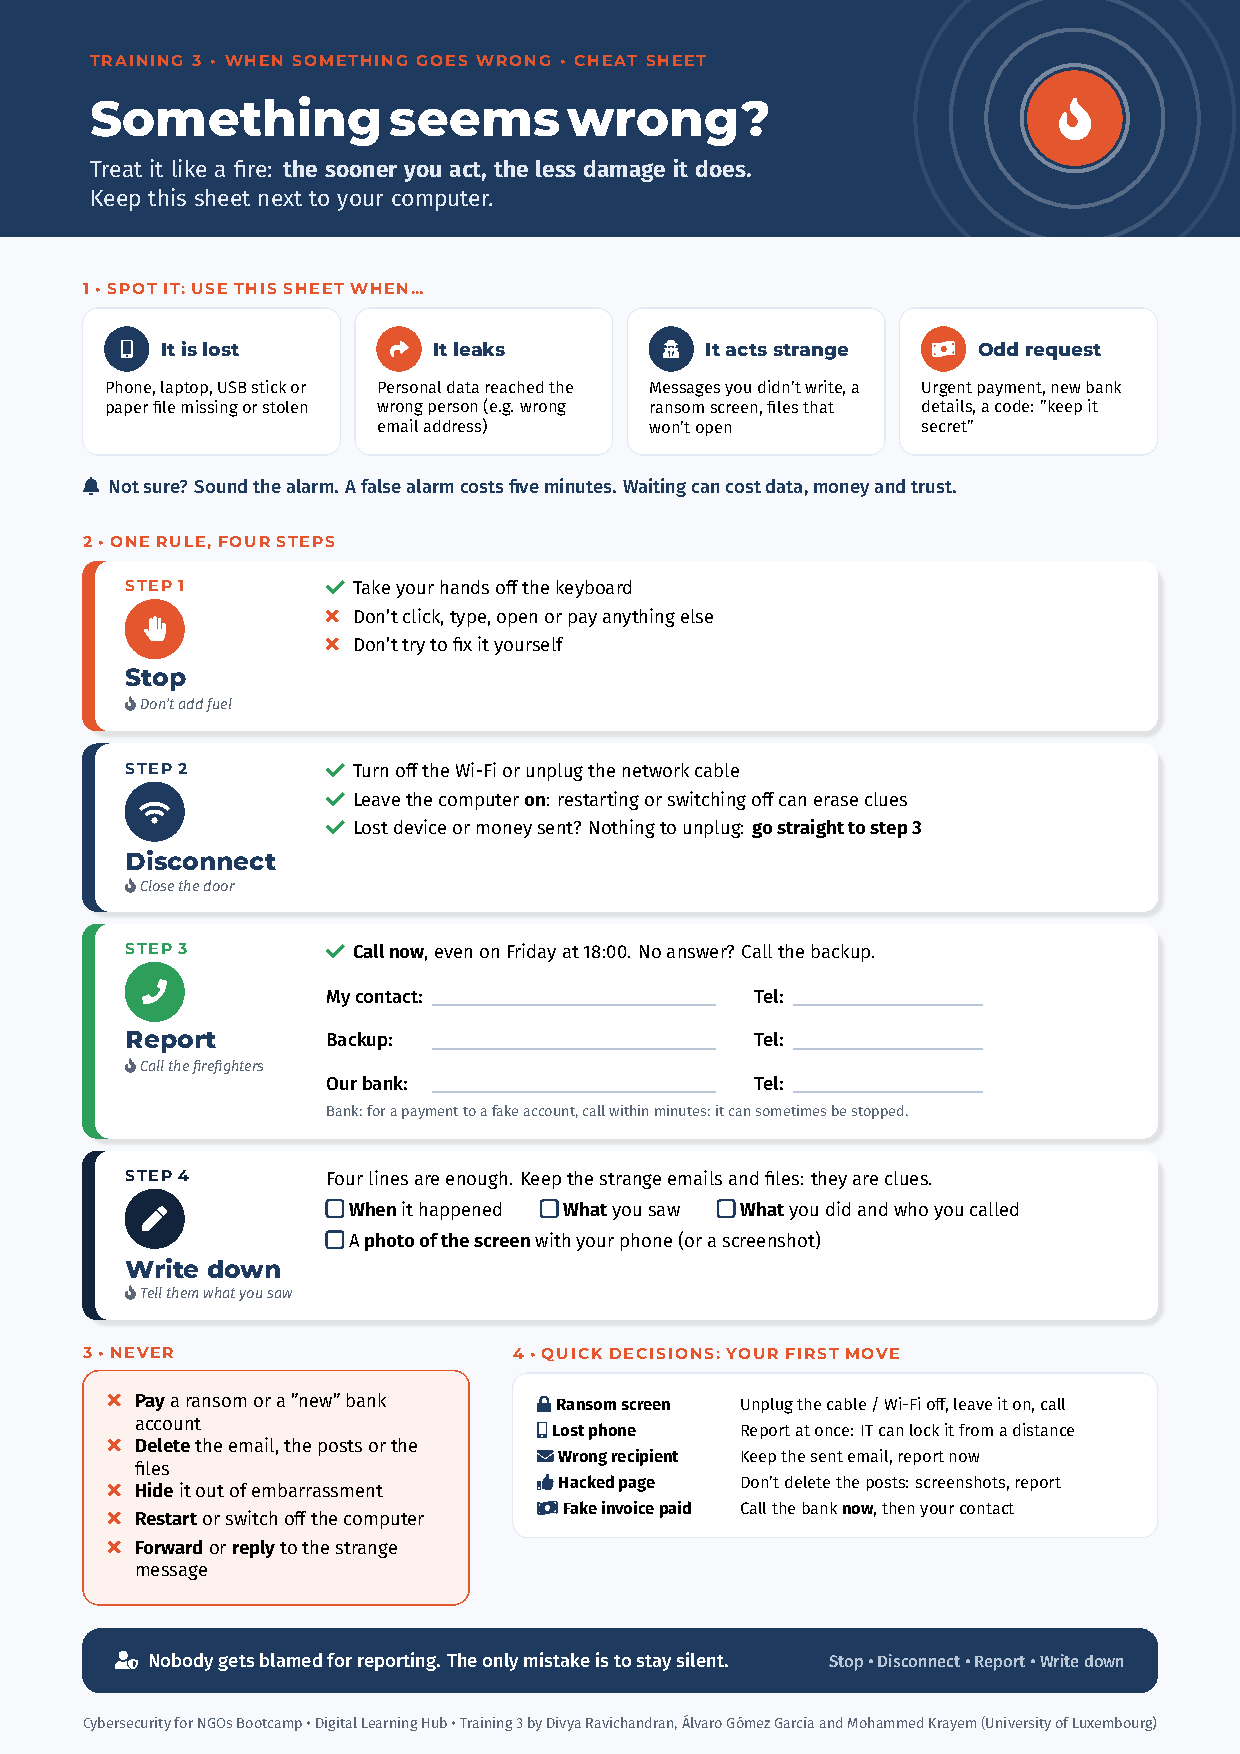
\includegraphics[height=50mm]{../05-take-home/cheat-sheet.pdf}};
    \column{.6\textwidth}
    \gstep{alert}{\faSearch}{\textbf{When to use it:} lost, leaked, acting strange, odd request}
    \gstep{navy}{\faListOl}{\textbf{The four steps}, with what to do and what not}
    \gstep{good}{\faPen}{\textbf{Today:} write the names and numbers of your contact, your backup and your bank}
    \gstep{alert}{\faTimes}{\textbf{Never:} pay, delete, hide, restart, forward}
  \end{columns}
  \note{Hand out the cheat sheet (05-take-home/cheat-sheet.pdf); online, share the PDF in the chat. Ask everyone to
  fill in the three phone numbers before they leave or today: it is the most useful minute of the training. (~1.5 min)}
\end{frame}

% ---------- 31 · Key messages ----------
\begin{frame}{Remember three things}{Key messages}
  \vspace{0mm}
  \begin{columns}[T,onlytextwidth]
    \column{.31\textwidth}
    \takeaway{navy}{\faFire}{It's like a fire}{Spot it early: the sooner you act, the less damage}
    \column{.31\textwidth}
    \takeaway{alert}{\faListOl}{One rule}{Stop, Disconnect, Report, Write down}
    \column{.31\textwidth}
    \takeaway{good}{\faUserShield}{No blame}{Never pay, delete or hide. Not sure? Sound the alarm}
  \end{columns}
  \vspace{1mm}
  \centering{\mediumfont\color{navy}\faComments\ \ Feedback: one thing you liked, one thing to improve (aloud or in the chat)\par}
  \note{Recap in three sentences, then collect feedback: one thing they liked and one thing to improve, aloud
  or in the chat. (~1.5 min)}
\end{frame}

% ---------- 32 · Thank you ----------
{\darkslide
\begin{frame}[plain,c]
  {\kickerfont\fontsize{8}{10}\selectfont\color{alert}CYBERSECURITY FOR NGOS \textbullet{} TRAINING 3}\par\vspace{4mm}
  \begin{minipage}{112mm}\raggedright
    {\headfont\fontsize{30}{35}\selectfont Thank you!\par}\par\vspace{4mm}
    {\lightfont\fontsize{14}{18}\selectfont\color{soft}Stop \textbullet{} Disconnect \textbullet{} Report \textbullet{} Write down}\par\vspace{9mm}
    {\small\color{soft}Divya Ravichandran \textbullet{} Álvaro Gómez García \textbullet{} Mohammed Krayem\\University of Luxembourg\par}\vspace{4mm}
    \pill{alert}{\faQuestionCircle\ Questions?}
  \end{minipage}
  \note{Thank everyone, answer last questions. On the trainer screen: Delete data once the CSV files are saved. (~30 s)}
\end{frame}
}

\end{document}
